
\chapter{Spatial analysis}



\pagestyle{fancy}

Analysis is one of the key capabilities of GIS. Spatial analysis is the \textbf{quantitative analysis of phenomena, considering the geometric, geographical or topological properties of their elements}. Properties such as position, distance, or area are relevant when performing spatial analysis.

We perform spatial analysis when we use a classic printed map to search for the highest peak in a given map sheet, read the elevation of a given element such as a city, or plan a turistic activity checking the places to visit and how to move between them using the best roads or following the fastest route. Of course, we can also perform this kind of operations within a GIS.

Analysis generates new data, and that data can be in the form of \textbf{new layers, tables, or simple values}.

The result of an analysis might express \textbf{the same variable} as the original data (for instance, computing the average value), or \textbf{a different one} (for instance, if we compute a slope layer from an elevation layer).

Spatial analysis requires spatial data, which can be of a \textbf{single type}, or, instead, of \textbf{multiple types that are combined}. For instance, in the case of finding the highest point in a map, the result is just a coordinate and the only variable used is the elevation. In the case of computing the average elevation of a city, two variables are used: the elevation and the space occupied by the city (defined, for instance, by a polygon with its boundaries). Although all that information is traditionally contained in a single map sheet, in a GIS they will be in separate layers, both if which will be inputs for this particular analysis.

Analysis in a GIS gives us answers to questions that can be:

\begin{itemize}
 \item Related to position or extension.
\item Related to shape or distribution.
\item Related to spatial associations.
\item Related to spatial interactions.
\item Related to spatial variation.
\end{itemize}

\section{Some examples of spatial analysis}

The following sections describe some common types of spatial analysis.

\subsection{Spatial queries}

We already discussed queries in the chapter devoted to databases.

Queries can be combined with other analysis tools, for instance, to \textbf{select} a subset of feature with which we will later perform some other analysis.

\subsection{Topological analysis}

Queries can be refered not just to the position of geographical elements, ut also to their \emph{relation with other elements}. If we have topological information, we can perform analysis that responds to questions such as:

\begin{itemize}
\item How can I reach a give coordinate from my current position using the existing road network? 

\item Which countries share their border with France?
\end{itemize}

\subsection{Measurement} 

Spatial properties can be quantified and measured. Among the most basic ones, we find length, area, perimeter or shape factors. More elaborated ones such as slope or multiple indices derived from basic masurements can also be computed with the help of a GIS.


\subsection{Combination}

One of the most typical procedures within a GIS is the \tetbf{combination and overlay} of layers. The separation of geographical data into layers facilitates this kind of operations, and turn GIS into the optimal platform to perform any analysis that requires combining information from different variables.

In the case of vector layers, overlay operations such as \textbf{union, intersection, difference or clipping} are frequently used. Figure \ref{Fig:Intersection} shows an example of an overlay operation between polygon layers.

\begin{figure}[!hbt]   
\centering
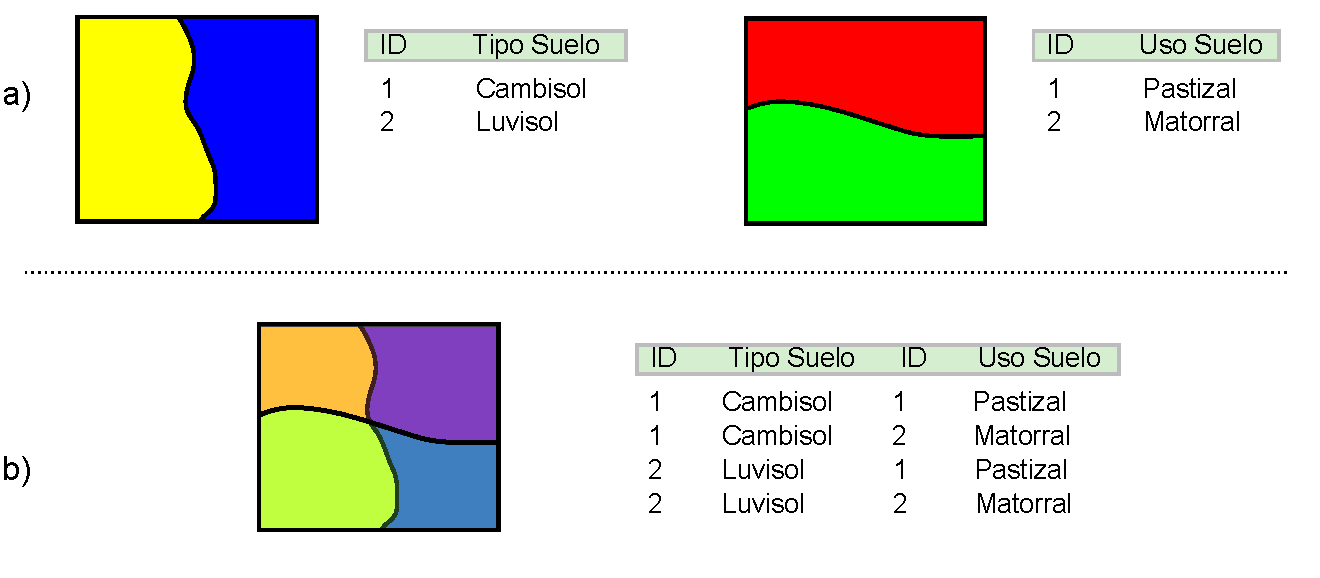
\includegraphics[width= \columnwidth]{Analysis/Intersection.pdf}
\caption{\small Intersection between two polygon layers.}
\label{Fig:Intersection} 
\end{figure}

\subsection{Transformations}

We include in this group a large set of operations that alter the input data in different ways. Among them we find \textbf{coordinate transformations}, \textbf{simplification of geometries} or the \textbf{creation of influence areas (buffers)}. These transformations may affect both the spatial component and the thematic component of the data. 

A particular case, already mentioned in a previous chapter, is the \textbf{conversion between representation models}. Figure \ref{Fig:Conversions} shows an example of this. Starting with a scanned map (a raster layer) with contour lines, these can be traced and a vector layer created based on them. The lines in that vector layer can be later converted into a raster DEM using interpolation techniques. From the raster DEM it is possible to obtain contour lines at an arbitrary contour distance (of course, within the level of detail of the original data).

\begin{figure}[!hbt]   
\centering
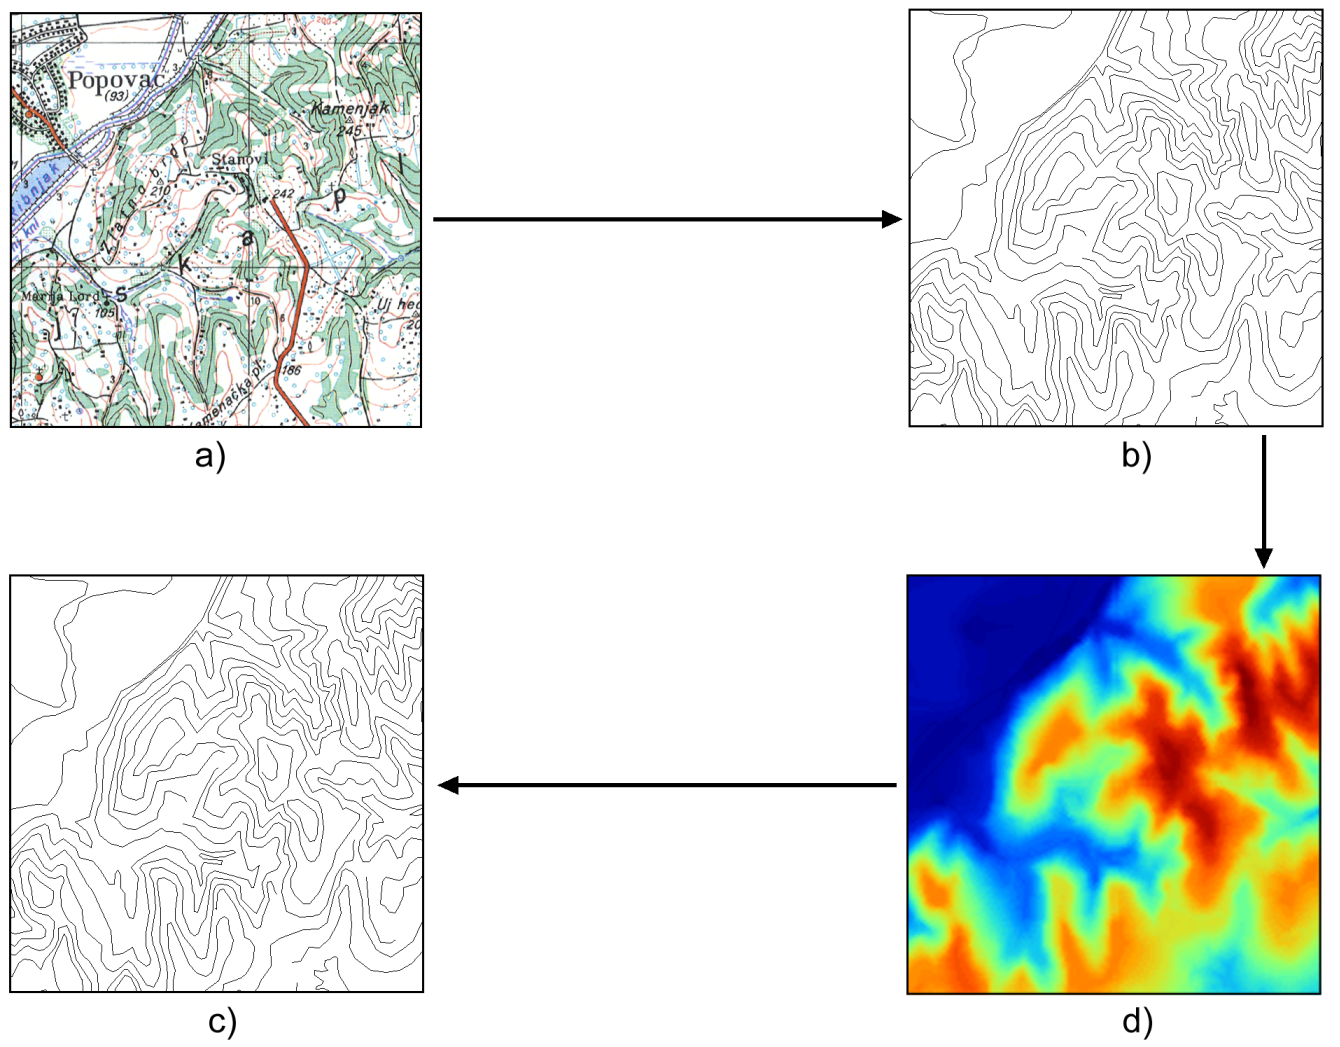
\includegraphics[width= \columnwidth]{Analysis/Conversions.png}
\caption{\small Conversion between representation models for an elevation layer.}
\label{Fig:Conversions} 
\end{figure}

\subsection{Terrain analysis}

Terrain analysis is one of the most powerful capabilities we find in GIS. From basic parameters such as \textbf{slope} or \textbf{aspect}, to highly specific morphometric ones, and passing through a large collection of tools for \textbf{hydrological analysis}, a vast array of analysis capabilities is available in this field.

\subsection{Descriptive statistics}

The common elements of classic statistics have their equivalents when working with geographical data, and they allow us to \textbf{quantitatively describe} the data we work with. Here we include centrality and dispersion measures,  pattern analysis, and many others. These can be themselves used in hypothesis testing, in case there is a spatial component involved.

These statistical values allow us to respond to questions such as:


\begin{itemize}
\item Is average height a constant value across a given country?

\item Is there a predominant movement direction for individuals of a given species, or do they move erraticaly?
\end{itemize}

\subsection{Inference}

Another important statistical analysis in GIS is the one that helps infering the behaviour of variables and their evolution.

\tetbf{Change modelling} is one of the many fields that are rapidly evolving thanks to the help of GIS.

\subsection{Optimization and decision-making}

The layered structure of geographical information in a GIS, which, as we have seen was ideal for overlay operations, provides also an optimal framework for estudied the combined effect of multiple platforms. GIS is the perfect framework for \tetbf{multiple-criteria analysis}.

Questions such as the following ones can be responded using a GIS:

\begin{itemize}
\item Which one is the best place to build a new pwer station considering its effect on the environment and the people living close to it?

\item Where should a hospital be located to provide the best possible service to the inhabitants of a given region?
\end{itemize}


\section{Particularities of spatial data for its analysis}

Spatial data has some great potential thanks to its particular properties, but at the same time these properties might \tetbf{limit or condition} working with them. In some cases, they might represent problems that have to be considered when analyzing them; in others, they are just something that anyone working with them should know, but that are not problematic \emph{per se}.

\subsection{Scale}

We can study geographical information at \emph{different scales}, and depending one we use, the results we will otain will be different. For this reason, apart from considering scale when rendering and visualizing geographical data, the \textbf{analysis scale} should be considered as well when performing any analysis.

The analysis scale should depend on the \emph{data properties} (accuracy, data type, etc.) and the \textbf{analysis to be performed} with them.

This can be easily understood with the help of \ref{Fig:Scales}. If we want to categorize the form of terrain at a given point, we need to analize the elevation of the point and also the elevation in its surroundings. Depending on the size of that analysys <<window>> around the center point (which is what defines the analysis scale), the results can be very different. In the image, for a small value of the analysis radius, the terrain will be categorized as being a peak. For a larger region, however, it will be considered the bottom of a valley.



\begin{figure}[h]   
\centering
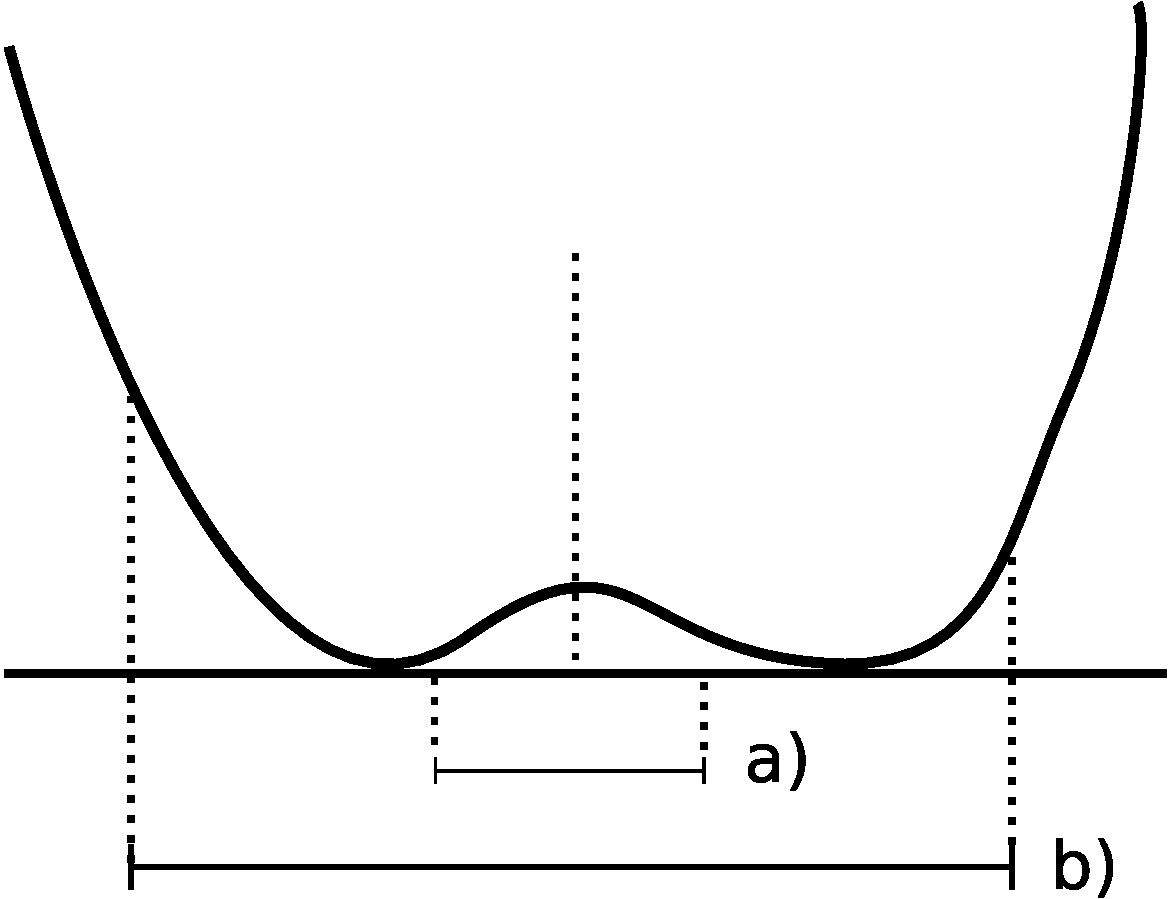
\includegraphics[width= .45\columnwidth]{Analysis/Scales.pdf}
\caption{\small Depending on the analysis scale, the form of the terrain can   be classified as a peak (a) or a valley bottom (b).}
\label{Fig:Scales} 
\end{figure}

Therefore, we must <<look>> at the terrain at the correct distance for which the information that it gives us is the most interesting and correct for the kind of analysis that we are performing. Apart from the fact that there is an optimal analysis scale for each type of analysis, it is also interesting to work at \textbf{multiple scales}, since that will provide us more information than what we can obtain working only at a single scale.

Another example of how the analysis scale affects the analysis result is found in the case of \textbf{taking measurements}. As it can be seen in figure \ref{Fig:Fractal_line}, the measurement unit (which is implicitely defined by the level of detail of the data) that is used causes the results to be different. 

\begin{figure}[h]   
\centering
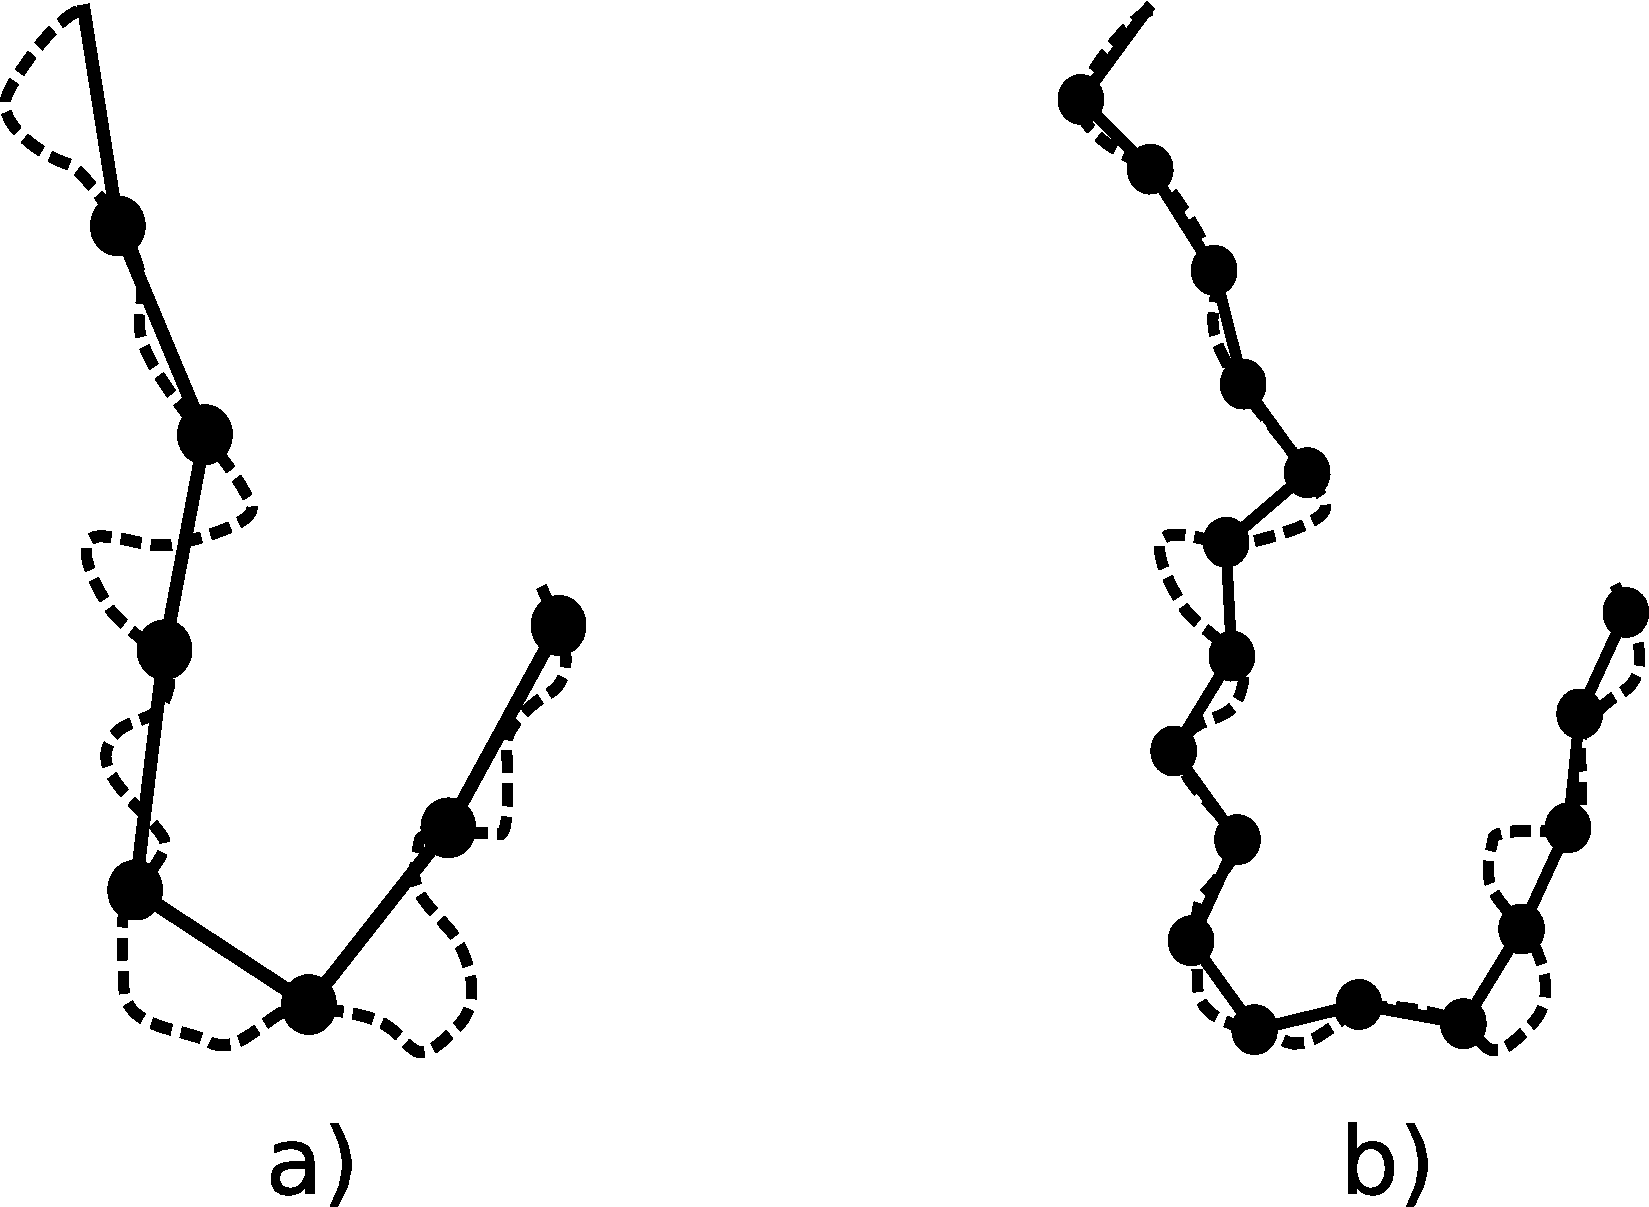
\includegraphics[width= .45\columnwidth]{Analysis/Fractal_line.pdf}
\caption{\small Measurement unit affects the value of the measurement.}
\label{Fig:Fractal_line} 
\end{figure}

A vlue by itself might not have mening if it is not accompanied by the scale that was used to obtain it.

The concept of \textbf{fractal} has a direct link with this.


\subsection{The Modifiable Areal Unit Problem}


Many of the variables that with which we work in a GIS \textbf{cannot be measured at a single point}, and they must be \textbf{aggregated for a given area around that point}. Examples of that are the percentage of the population within a given age range, or the population density. 

Areas defined to work with these variables are \textbf{esentially arbitrary}, such as countries, counties, districts, etc., and they are defined without taking into account any criteria related to spatial anlysis. Using different areas (different units for computing the values of the variable) will yield different results.

This problem is known as the \textbf{Modifiable Areal Unit Problem} (PUAM). Solving or reducing its effect is complex, and no solution exists that can be applied in all cases, but whenever we work with this type of geographical data, it is important to keep in mind that there will be a source of statistical bias that cannot be neglected.

Another problem relateb with the PUAM is the so-called \textbf{ecological fallacy}, which result from (wrongly) assuming that the values computed for a given area can be assigned to the individuals of the population within that area. This would be true only in the case of complete homogeneity.


\subsection{Spatial autocorrelation} 

\textbf{Spatial autocorrelation} is the \tetbf{correlation of a variable with itself}, in such a way that values of the variable at any point are correlated with values of that same variable in close-by points. For instance, in the case of temperature, points close to a heat source will have a higher temperature that those far from it or closer to a cold spot. If we study the distribution of an infectious disease, reported cases are likely to appear grouped, and a large number of them normally cause the neary populations to also be largely affected by the disease.

Another way of expressing this is using the well-known \textbf{Tobler's First Law of Geography}, which states that <<everything is related to everything else, but near things are more related than distant things>>.

In the above cases, sppatial autocorrelation is said to be \textb{positive}. However, it can be also \textbf{negative}, if higher values are surrounded by lower ones, or there can be no correlation at all, when values in separate points are \textbf{independent} and do not affect each other regardless of distance.

Figure \ref{Fig:Autocorrelation} shows three raster layers which demonstrate the above types of spatial autocorrelation.

\begin{figure}[!hbt]   
\centering
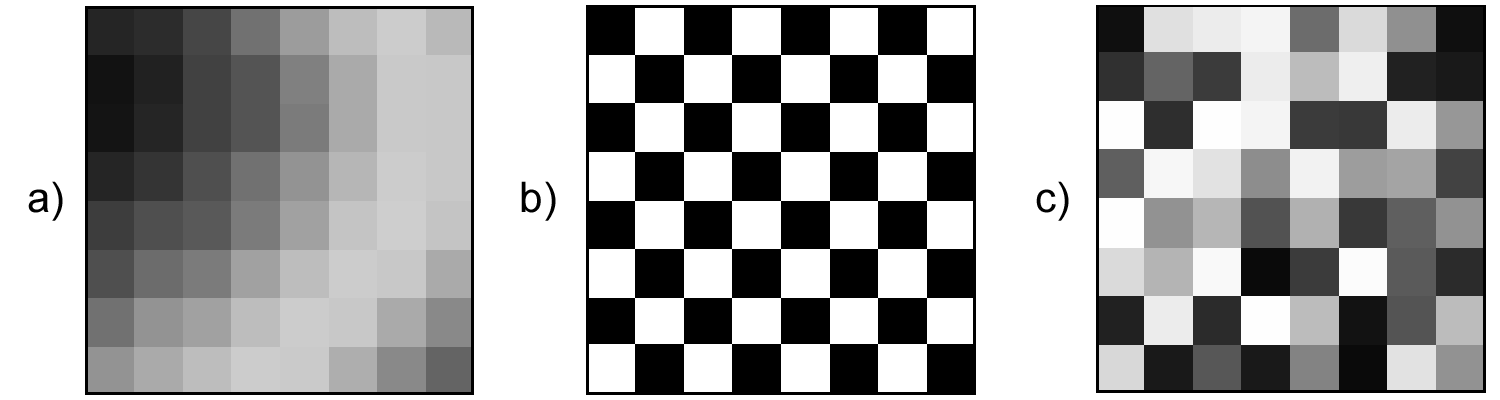
\includegraphics[width=\textwidth]{Analysis/Autocorrelation.png}
\caption{\small a) Positive spatial autocorrelation. b) Negative spatial autocorrelation. c) No spatial autocorrelation (independency).}
\label{Fig:Autocorrelation} 
\end{figure}

The existence of spatial autocorrelation has many important consequences.

First, many of the most commmon statistical analyses assume depency of the variable that is being studied. Since there is a dependency on the spatial component, this component has to be introduced as another variable to consider, in order to ensure that results are sound.


Something similar happens when data have a \textbf{spatial trend}(values of a variable depend on the position, like, for instance, temperature values, which show a clear trend as latitude changes), since that also invalidates the assumption that data are independent.

If positive correlation exists, \textbf{statistical inference is less effective}. The same number of observations contain less information about the phenomena represented by the variable.

The consequences of spatial autocorrelation, however, are not only negativa. If points located in the vicinity of a given one are related to it, and the value of a variable are affected by that proximity, that can be used to \textbf{estimate values} at any point, knowing the values in a set of naerby points. That is the fundamental idea behind \textbf{interpolation methods}.


\subsection{Structure}

Both the data itself and the properties of the phenomeon they represent (such as the aforementioned spatial correlation) have some sort of structure. This structure can have a relevant effect on the analysis results, and should be taken into account.

The two basic statistical concepts related to the spatial structure of a process are \textbf{stationarity} and \textbf{isotropy}. Stationarity indicates that the process is \textbf{translation-invariant}. That is, its properties are constant across the whole space and there is no spatial trend. Isotropy means that the process is \textbf{rotation-invariant}, and happens in the same way in all directions.

\subsection{Border effects}

The areas in which we perform spatial analysis \textbf{have boundaries}. These might be artificial ---for instance, the limit of the aerial photograph we are working with---, or natural ---if we study a forest that is close to a lake, the shore will be limit of the forest. Boundaries \tetbf{distort the result of analysis}, specially for those variables that have to be aggregated (density, etc., as we saw for the case of PUAM)

In some cases, the border effect might manifest itself only for those point close to the border. In others, however, \textbf{all the points related or somehow connected to the border} might be affected, regardless of the distance to it.

\pagestyle{empty}